\subsection{\acl{BDD}}
\label{subsec:bdd}

%Research has conducted extensive analysis on the failure of software development projects. Notable studies, such as the 2015 Chaos Report by the Standish-Group\footnote{https://standishgroup.com/sample\_research\_files/CHAOSReport2015-Final.pdf}, indicate that 44\% of the analyzed projects did not meet their targets, and a 2012 McKinsey study reveals that software projects typically deliver 17\% less value than anticipated \cite{bloch2012delivering}. A widely recognized contributing factor to this shortfall is the absence or inadequacy of requirements defined by end-users and domain experts \cite{al2009taxonomy,cerpa2009did,linberg1999software,pinto1990causes}.


\acf{BDD} is a software development practice intricately woven into the framework of agile methodologies, signifying a profound transformation in conventional software engineering approaches. It positions itself as a dynamic response to prevalent challenges by prioritizing user behaviors and aligning closely with business needs. Rooted in the integration of concepts from both \ac{TDD} and \ac{DDD}, \ac{BDD} transcends traditional development paradigms.

\ac{BDD} stands out as a departure from the typical \ac{TDD} methodology, where the primary focus is on writing tests for isolated code units, with a predominant technical viewpoint. Instead, \ac{BDD} broadens its perspective, bridging the gap between technical and business aspects. It achieves this by incorporating viewpoints from both spheres, redirecting the evaluation from individual code segments to the holistic assessment of the application's behavior from the user's standpoint. This strategic shift not only enhances communication but also fosters collaboration among developers, testers, and business stakeholders, as evidenced by prior research~\cite{smart2023bdd,pereira2018behavior}.

In response to the challenges posed by the highly technical and code-centric nature of \ac{TDD}, \ac{BDD} introduces an innovative testing methodology. Rooted in a user-centric philosophy, test cases are structured using a language that mirrors natural language. This linguistic clarity serves as a catalyst for effective collaboration, ensuring a shared understanding among team members throughout the software development lifecycle.

\subsection{Gherkin}
\label{subsec:gherkin}

Gherkin is a \ac{DSL} prominently utilized in the domain of \ac{BDD}. It is employed for crafting requirements and tests in a clear, human-readable format. Gherkin's syntax follows a systematic Given-When-Then structure, interweaving natural language expressions, as demonstrated in \cref{lst:withdrawcash}. Therefore, focusing on the end-user's perspective and business requirements rather than the underlying technical implementation.

\begin{listing}[!ht]
\caption{Examplary feature file with one scenario}
\label{lst:withdrawcash}
\inputminted{gherkin}{files/code/atm.feature}
\end{listing}

 Gherkin employs a distinct set of keywords to delineate various facets of test scenarios. Notably, it utilizes the \textit{Feature} keyword to expound upon the primary functionality of the feature under examination, \textit{Scenario} for specifying individual use cases within the feature, \textit{Given}-steps to establish initial context or preconditions, \textit{When}-steps for denoting the event or action triggering the scenario, and \textit{Then}-steps for articulating anticipated outcomes for validation\footnote{It is imperative to acknowledge that this chapter does not exhaustively cover all Gherkin keywords, but rather focuses on those pertinent to our study. A comprehensive list is available at \href{https://cucumber.io/docs/gherkin/reference/\#keywords}{https://cucumber.io/docs/gherkin/reference}}. Furthermore, the \textit{And} keyword facilitates the chaining of multiple steps of the same type, ensuring a logically granular and encapsulated representation of test steps. This structural arrangement cultivates a shared understanding among stakeholders concerning the expected system behavior, thereby mitigating the previously delineated structural challenges. Notably, this structure harmonizes well with user stories and other agile methodologies, presenting sufficient structure for interpretation by frameworks such as Cucumber to map individual test steps to executable code (cf.~\cref{subsec:cucumber}).


\subsection{Cucumber}
\label{subsec:cucumber}

Following the introduction of \ac{BDD} in \ref{subsec:bdd} and the Gherkin \ac{DSL} in \ref{subsec:gherkin}, it is essential to understand how these high-level scenarios are mapped to executable code. Consider \cref{fig:cucumber-mapping}:

\begin{figure}
    \centering
    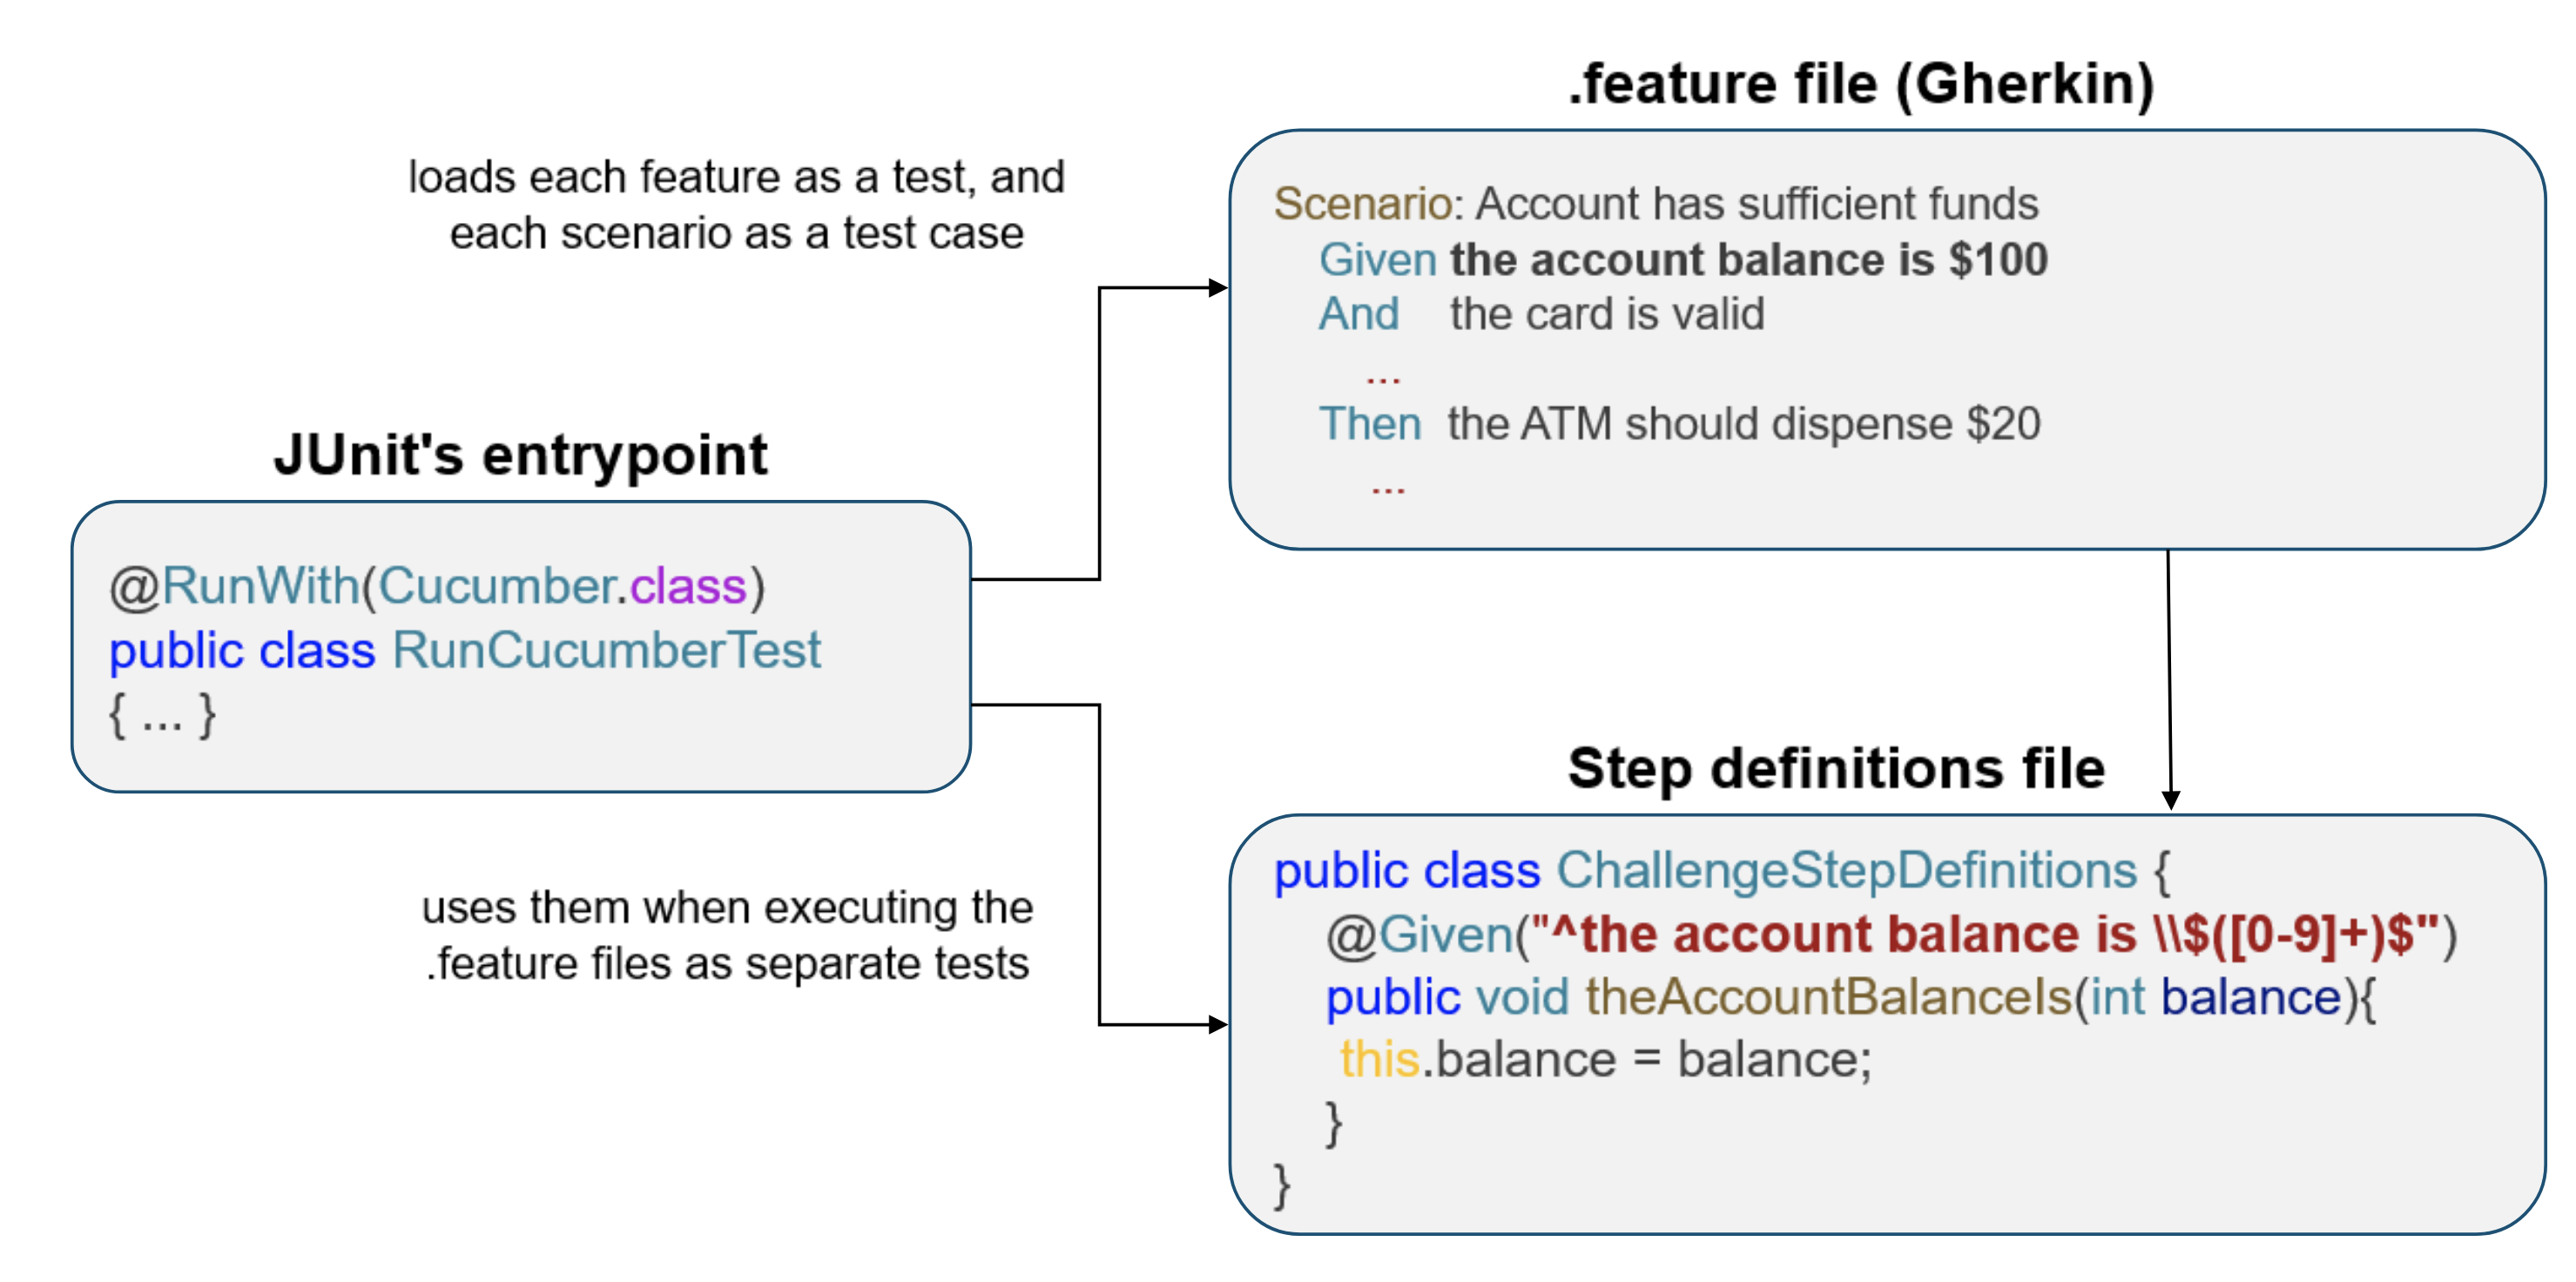
\includegraphics[width=\linewidth]{files/figures/cucumber_test_step_mapping.png}
    \caption{Cucumber test step mapping}
    \label{fig:cucumber-mapping}
\end{figure}

Expanding on the initial scenario presented in \cref{lst:withdrawcash}, the corresponding figure (\cref{fig:cucumber-mapping}) illustrates the link between the specified test steps and their concrete code representations. This connection is primarily established through the use of pattern matching via regular expressions. For instance, consider the function \textit{theAccountBalanceIs}, marked with the Cucumber-specific \textit{@Given} annotation that includes a \ac{Regex}. When a test step is executed, and its type (e.g., Given, When, Then) aligns with the annotation of the function as well as the pattern defined by the \ac{Regex}, the respective function is fired, leading to the execution of its underlying code. By assigning values to instance variables, cucumber can handle a shared context in a scenario across test steps, thus enabling a consistent and continuous testing flow.

Drawing upon the examples and principles detailed in this chapter, it becomes evident that \ac{BDD}, with its emphasis on clear, collaborative communication across stakeholders and its ability to seamlessly integrate user-defined scenarios with automated testing, represents a significant advancement in aligning software development processes with both business requirements and user expectations.

\subsection{Distributed Systems}
\label{subsec:dissys}
A distributed system is a network of independent computers, running on multiple servers or nodes, that interact and synchronize their activities through the exchange of messages \cite{tanenbaum2007distributed}. These systems consist of components that collaboratively work towards a shared objective, presenting advantages in terms of performance, scalability, and redundancy when compared to centralized systems. The shift towards distributed systems is motivated by the inadequacies of non-distributed, centralized computing models, typified by a single monolithic server. Such centralized models have proven insufficient in addressing the increasing computational requirements and the need for enhanced system capabilities that could not be mitigated by vertically scaling a single system.

The distinctive feature of distributed systems lies in their avoidance of shared computing and memory resources, introducing complexities related to heterogeneity, scalability, and failure handling, among other challenges~\cite{coulouris2005distributed}. Non-distributed systems may struggle to effectively manage these challenges, leading to limitations in performance, scalability, and fault tolerance. Distributed systems, by distributing computational tasks across a network of interconnected computers, address these shortcomings.

For instance, consider a scenario where a centralized system, operating on a single powerful server, reaches the maximum capacity of available hardware resources. Upgrading the hardware of that single machine (vertically scaling), may become impractical or cost-prohibitive. In such situations, distributed systems offer a viable solution. By distributing the workload across multiple interconnected nodes, these systems enable parallel processing, allowing for efficient utilization of available resources beyond the constraints of a single machine. 

\subsection{\acl{RCE}}
\label{subsec:rce}

\ac{RCE} is an open-source application primarily developed at the \ac{DLR}. It is designed to facilitate the multidisciplinary engineering process, especially in complex system engineering such as aerospace, enabling users to integrate various disciplinary tools, define dependencies between them, and execute multidisciplinary workflows\cite{BODEN2021100759}. A key feature of \ac{RCE} is its capability to connect different \ac{RCE} instances in a distributed systems manner, which greatly facilitates collaboration across various departments and specializations. This interconnected approach allows engineers from multiple disciplines to contribute their individual tools to a unified workflow, enhancing efficiency and reducing the propensity for errors in complex engineering projects. In this paper, our focus will be limited to those aspects of \ac{RCE} that are relevant to our project. Consequently, many features and advantages of \ac{RCE} that extend beyond the scope of our work will not be addressed herein. For a comprehensive presentation of \ac{RCE} as well as its capacity to facilitate multidisciplinary collaboration, the reader is directed to consult the detailed tool papers provided in \cite{BODEN2021100759,boden2019distributed}, which offer extensive insights into the broader applications and benefits of \ac{RCE}.

% RCE (Remote Component Environment) is an open source software that helps engineers, scientists and others to create, manage and execute complex calculation and simulation workflows. A workflow in RCE consists of components with predefined inputs and outputs connected to each other. A
% component can be a simulation tool, a tool for data access, or a user-defined script. Connections define
% which data flows from one component to another. There are predefined components with common
% functionalities, like an optimizer or a cluster component. Additionally, users can integrate their own
% tools. RCE instances can be connected with each other. Components can be executed locally or on
% remote instances of RCE (if the component is configured to allow this). Using these building blocks,
% use cases for complex distributed applications can be solved with RCE.~\cite{rceDevGuide10x}